\scanpage{358}
\diagram{\begin{tikzcd}
K(Z,i)\timesK(Z,j)\arrow[r]\arrow[d]&K(Z,i+j\\
K(Z,i)\otimesK(Z,j)\arrow[ur,"f"']&{}
\end{tikzcd}}

Il suffit de construire $Nf$
\diagram{\begin{tikzcd}[column sep=large]
N(K(Z,i)\otimesK(Z,j)\quad\cdot\arrow[dr,"\text{E.Z.}"']&&NK(Z,i+j)=Z[i+j]\\
&NK(Z,i)\otimes NK(Z,j)\arrow[ur]&{}\\
&Z[i]\overset{\Vert}{\otimes}Z[j]&{}
\end{tikzcd}}

% Deleted block: the two large diagonal strokes cross the entire parenthesized diagram.
\figure{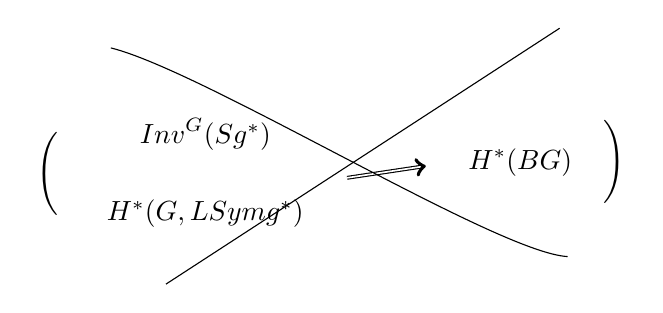
\begin{tikzpicture}
\node(a) at (0,1) {$\operatorname{Inv}^G(Sg^*)$};
\node(b) at (0,0) {$H^*(G,L\operatorname{Sym}g^*)$};
\node(c) at (4,.65) {$H^*(BG)$};
\node at (-2,.5) {$\Bigg($};\node at (5.2,.65) {$\Bigg)$};
\draw[double,->](1.8,.45)--(2.8,.6);
\draw(-1.2,2.1) .. controls (0,1.8) and (3.7,-.5) .. (4.6,-.55);
\draw(-.5,-.9)--(4.5,2.35);
\end{tikzpicture}}
\mspage{359}
